\chapter{Détermination du diamètre optimal des intervalles à considérer pour l'estimation de la régularité locale }
\minitoc%


Nous avons désormais établi que la génération d'un $\operatorname{FAR}(1)$ basé sur un mouvement brownien multi-fractionnaire permettait de contrôler de bout-en-bout la régularité du processus. Ceci va nous permettre de pouvoir analyser correctement le comportement du risque d'estimation de la régularité en fonction de $\Delta$, ainsi que le comportement du $\Delta^*$ optimal.

\section{Choix des paramètres de la simulation des $\operatorname{FAR}(1)$ localement Hölderiennes}

\info{
	Il est conseillé de se référer aux tableaux [Notations-Spécifique au stage]
	%\ref{tab:notation-specifique-stage} 
	et \ref{tab:model} pour la signification des notations déjà introduites et utilisées dans ce chapitre.
}

\subsection{Nombre de simulations}

Afin d'étudier la relation entre le $\Delta$ optimum et différentes quantités caractéristiques aux données, on va effectuer une simulation de monte carlo.

On décide de générer $\mathsf{mc} = 200$ simulations de Monte-Carlo, afin d'obtenir les résultats les plus robustes possibles pour l'estimation du risque $\esperance{\distnorme 2 {\widehat \Theta} {\widetilde \Theta}}$, tout en gardant un temps de calcul raisonnable. On fait varier $\lambda$ de $30$ à $480$ en incrémentant de $15$ à chaque fois. L'idée et de pouvoir regarder si il existe une relation entre $\Delta^*$ et la position du nombre moyen de points observés apr courbe $(\lambda)$ par rapport au nombre de courbes $(N)$.

\smallskip

Il est possible de voir comment les paramètres que l'on va définir sont utilisés dans l'implémentation en annexe \ref{annexe:code}.


\newcommand{\tlnm}{T^{[\lambda]}_{n}[m]}
\newcommand{\mset}{\llbracket 1, M_n \rrbracket}
\newcommand{\nset}{\llbracket 1, N \rrbracket}
\newcommand{\lbdset}{\llbracket 30, 45, \dots , 480 \rrbracket}
\newcommand{\genxset}{\bigl(\tlnm, X_n(\tlnm)\bigr)_{m \in \mset}}
\newcommand{\simset}{\left\{ \genxset \, : \, n \in \nset, \, \lambda \& N \textsf{ fixés } \right\}}
\newcommand{\simsetall}{\left\{ \genxset \, : \, N \in \overrightarrow N, \, \lambda \in \lbdset, \, n \in \nset \right\}}

\subsection{Fonction de Hurst}

\begin{minipage}{0.47\linewidth}
	On appelle $H : t \mapsto H_t$ la fonction de Hurst. Celle qui a été choisie est la suivante :

	$$
		H^{[0.4, 0.8, 5, 0.5]}_{\textsf{logistic}} : \begin{array}{ccc}
			[0,1] & \longrightarrow & [0.4, 0.8]
			\\
			t     & \longmapsto     & 0.4 + \frac{(0.8 - 0.4)}{1 + e^{-5(t - 0.5)}}
		\end{array}
	$$

	On dispose donc d'une régularité locale qui varie sur $\mathcal T$, tout en ayant une évolution pas trop brusque. Nous allons étudier le comportement du $\Delta$ lors de l'estimation de la régularité locale en les points suivants :

	$$
		\vec t = \begin{bmatrix} 0.3 \\ 0.4 \\ 0.5 \\ 0.6 \\ 0.7 \\ 0.8 \end{bmatrix}
		\quad\quad
		H(\, \vec t \,) =
		\begin{bmatrix}
			0.51 \\ 0.55 \\ 0.6 \\ 0.65 \\ 0.69 \\ 0.73
		\end{bmatrix}
	$$

\end{minipage}
\hfill
\begin{minipage}{0.47\linewidth}
	\begin{figure}[H]
		\centering
		\begin{tikzpicture}
			\begin{axis}[
					width=\textwidth,
					xlabel=$t$,
					ylabel={$H^{[0.4, 0.8, 5, 0.5]}_{\textsf{logistic}}(t)$},
					xmin=0, xmax=1,
					ymin=0.4, ymax=0.8,
					axis lines=center,
					axis on top=true,
					domain=0:1,
					samples=100,
					legend style={at={(0.5,-0.15)},anchor=north},
					legend entries={Fonction de Hurst, Points d'estimation de la régularité locale},
				]
				\addplot [mark=none,smooth,blue] {0.4 + (0.8 - 0.4)/(1 + exp(-5*(x - 0.5)))};
				\addplot [only marks,mark=*] coordinates {
						(0.3,0.51)
						(0.4,0.55)
						(0.5,0.6)
						(0.6,0.65)
						(0.7,0.69)
						(0.8,0.73)
					};
			\end{axis}
		\end{tikzpicture}
		\caption{Hurst Function : Logistic}
		\label{plot:hurst-logistic}
	\end{figure}
\end{minipage}


\subsection{Constante de Hölder
}

On décide de simuler des mouvements browniens multi-fractionnaires de constante de Hölder $L_t$ identique sur tout le support.

$$\forall t \quad L_t = 1$$


\subsection{Moyenne}


\begin{minipage}{0.47\linewidth}

	La fonction moyenne du processus utilisée pour la simulation est la suivante :

	$$
		\mu : \begin{array}{ccc}
			[0,1] & \longrightarrow & \mathbb R
			\\
			t     & \longmapsto     & 4 \cdot \sin\bigl( \frac 3 2 \pi \cdot t \bigr)
		\end{array}
	$$
\end{minipage}
\hfill
\begin{minipage}{0.47\linewidth}
	\begin{figure}[H]
		\centering
		\begin{tikzpicture}
			\begin{axis}[
					width = \textwidth,
					xlabel=$t$,
					ylabel=$\mu(t)$,
					xmin=0, xmax=1,
					ymin=-4, ymax=4,
					axis lines=center,
					axis on top=true,
					domain=0:1,
					samples=100
				]
				\addplot [mark=none,smooth,blue] {4*sin(deg(3/2*pi*x))};
			\end{axis}
		\end{tikzpicture}
		%\caption{Mean function : $\mu(t) = 4 \cdot \sin\bigl( \frac 3 2 \pi \cdot t \bigr)$}
		\label{plot:mu}
	\end{figure}
\end{minipage}







\subsection{Noyau de la relation FAR(1)}
\begin{minipage}{0.48\linewidth}
	On décide de simuler un FAR(1) basé sur un opérateur linéaire intégral :

	$$
		X_{n+1} = \phi(X_n) + \varepsilon_{n+1}
	$$

	avec : $\phi : f \mapsto \displaystyle\int_{\mathcal T} f(u) \beta(u, \cdot \,) \, du$

	C'est une modélisation fréquente des FAR(1). Le noyaux que l'on considère dans l'opérateur intégral pour les simulations est le suivant :


	$$
		\beta : \, \begin{array}{ccc}
			[0,1]^2 & \longrightarrow & \mathbb R
			\\
			(t,s)   & \longmapsto     & \frac 9 4 t\sqrt{ s(1-s) }
		\end{array}
	$$

\end{minipage}
\hfill
\begin{minipage}{0.48\linewidth}
	\begin{figure}[H]
		\centering
		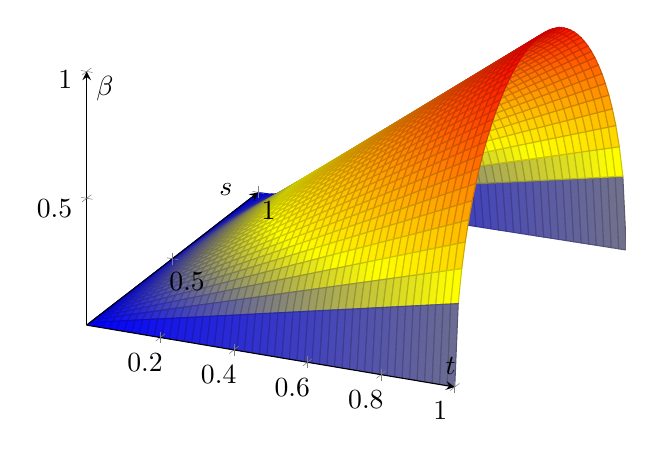
\begin{tikzpicture}
			\begin{axis}[
					xlabel=$t$,
					ylabel=$s$,
					zlabel=$\beta$,
					xmin=0, xmax=1,
					ymin=0, ymax=1,
					zmin=0, zmax=1,
					axis lines=center,
					axis on top=true,
					domain=0:1,
					samples=50,
				]
				\addplot3 [surf] {9/4*x*sqrt(y*(1-y))};
			\end{axis}
		\end{tikzpicture}
		\caption{Graphique du noyau intégral pour la relation FAR(1)}
		\label{graph:far_kernel}
	\end{figure}
\end{minipage}

\bigskip

On notera que le noyaux utilisé pour la relation de $\operatorname{FAR}(1)$ est une fonction lisse. Ainsi il remplit aisément la condition pour que le $\operatorname{FAR}(1)$ hérite de la régularité du mouvement brownien multi-fractionnaire généré.

\subsection{Nombre de courbes}

Afin d'étudier le lien potentiel qu'il pourrait y avoir entre le nombre de courbes observées et le $\Delta$ optimal pour l'estimation de la régularité locale, on choisit plusieurs valeurs de nombres de courbes observées de telle sorte à avoir un \og petit \fg et un \og grand \fg nombre de courbes observées.

On choisit les valeurs suivantes concernant le nombre de courbes observées :

$$
	\vec N = [ 100, 200, 300, 400]
$$

Ainsi on traîte les cas de ce qu'on pourrait considérer comme la limite avant d'entrer dans un cas \og sparse \fg (en terme du nombre d'observations de courbe), jusqu'à un nombre de courbe que l'on peut considérer important.

\subsection{Nombre moyen de points observés par courbe}

Le nombre de points observés sur la courbe $X_n$ est défini comme étant la variable aléatoire $M_n$. Dans le cadre de notre simulation, $M_n$ suit une loi de poisson de paramètre $\lambda$. Ainsi, $\esperance{M_n} = \lambda$ dans le cadre de notre simulation.

On effectue ainsi une simulation d'un échantillon de série temporelle $\operatorname{FAR}(1)$ par nombre moyen de points que l'on souhaite observer sur les courbes ($\lambda$). Afin de traîter différents cas, d'observation \og dense \fg à observation \og sparse \fg (dans le sens du nombre de points par courbe), on fait varier $\lambda$ de $30$ points par courbe en moyenne à $480$ points. L'idée est de voir ensuite si il y a une relation entre le $\Delta^*$ et le fait que l'on ait $\lambda$ petit, similaire ou grand par rapport à $N$.

\subsection{Ensemble des $\Delta$ testés}

On souhaite obtenir plusieurs graphiques avec $\Delta$ sur l'axe des abscisses afin de pouvoir étudier le comportement de diverses quantitées, dont le risque euclidien, lorsque l'on fait varier $\Delta$ avec certains paramètres fixés (nombre de courbes observées, nombre moyen de points observés par courbe, ...). Toutefois plus on va considérer de $\Delta$, et plus la simulation sera coûteuse. En effet, on a vu en section \ref{rem:inversion_matrice_covariance_mfbm_informel} que l'odre de complexité de la simulation du mfBm est de $\mathcal O \bigl( \operatorname{card} T^3 \bigr)$, avec $T$ les points où l'on doit évaluer nos $\famfinie X 1 n$. Dans notre cas, le nombre de points considérés pour la simulation est :

$$\underbracket[0.187ex]{\dim \vec\Delta}_{30} \times \underbracket[0.187ex]{3}_{t_1 / t_2 / t_3} \times \underbracket[0.187ex]{\dim \vec t}_{6} + \underbracket[0.187ex]{n_{Grid\_\int}}_{100} + \underbracket[0.187ex]{\lambda}_{\leq 480} \leq \underbracket[0.187ex]{640}_{fixe} + \underbracket[0.187ex]{480}_{pts \, aleat} = 1 \, 120$$

% Afin d'avoir une approximation correcte de l'intégrale requise pour la relation FAR(1), on choisit d'effectuer la méthode des rectangles en découpant $[0,1]$ en 100 sous intervalles réguliers. On a besoin aussi d'évaluer la vraie valeur des $X_i$ en $t_1, t_2, t_3$ et ce, pour chaque valeur de $\Delta$ afin de pouvoir comparer l'estimateur $\hat \theta(u,v) = \frac 1 N \sum_i (\widehat X_i(u) - \widehat X_i(v))^2$ obtenu via le pré-lissage avec la valeur intangible $\tilde \theta(u,v) = \frac 1 N \sum_i ( X_i(u) -  X_i(v))^2$; et ce sur l'ensemble des différents points $t_2 \in \vec t$


Pour assurer un équilibre entre le nombre de points et les temps de simulation, nous choisissons 30 valeurs uniformément réparties entre 0.01 et 0.2 pour $\Delta$. Au-delà de cette plage, la largeur des intervalles pour l'évaluation de la régularité devient disproportionnée par rapport à la taille du support, rendant inappropriée la notion de \og régularité locale \fg.
$$
	\vec \Delta = \left[ 0.01 \cdots  0.2 \right]_{30}
$$

\subsection{Bruit blanc}


Une fois que l'on a simulé :

$$
	\famfinie X 1 n \quad \textsf{vérifiant} \quad X_{n+1} = \phi(X_n) + \xi_n
$$

on doit désormais reproduire l'erreur de mesure, pour cela chaque courbe est ensuite bruitée en rajoutant un bruit blanc :

$$
	\eta \sim \mathcal N ( 0, 0.04 )
$$

Il est important d'avoir un bruit blanc d'écart type d'un ordre de grandeur en dessous de celui des valeurs prises par le processus, sinon l'estimation serait mauvaise quoi qu'il arrive. En effet le bruit écraserait à lui tout seul toute l'information fine de régularité.


\subsection{Résumé des Paramètres}

\begin{table}[H]
	\centering
	\begin{tabular}{l|l|ll|l|}
		\cline{2-5}
		\textbf{}                                                                  & \textbf{nombre de valeurs testées} & \multicolumn{1}{l|}{\textbf{de}} & \textbf{jusqu'à}         & \textbf{valeur}          \\ \hline
		\multicolumn{1}{|l|}{\textit{\textbf{$\Delta$}}}                           & $30$                               & $0.01$                           & $0.2$                    & \cellcolor[HTML]{C0C0C0} \\
		\multicolumn{1}{|l|}{\textit{\textbf{$\lambda$}}}                          & $30$                               & $30$                             & $480$                    & \cellcolor[HTML]{C0C0C0} \\
		\multicolumn{1}{|l|}{\textit{\textbf{$N$}}}                                & $4$                                & $100$                            & $400$                    & \cellcolor[HTML]{C0C0C0} \\
		\multicolumn{1}{|l|}{\textit{\textbf{Erreur de mesure : ($\sigma_\eta$)}}} & \cellcolor[HTML]{C0C0C0}           & \cellcolor[HTML]{C0C0C0}         & \cellcolor[HTML]{C0C0C0} & $0.2$                    \\
		\multicolumn{1}{|l|}{\textit{\textbf{nb simulations MC}}}                  & \cellcolor[HTML]{C0C0C0}           & \cellcolor[HTML]{C0C0C0}         & \cellcolor[HTML]{C0C0C0} & $200$                    \\ \hline
	\end{tabular}
	\caption{Hyper-paramètres de la simulation Monte-Carlo}
	\label{tab:hyperparam-mc}
\end{table}


\section{Prélissage des données simulées}

\subsection{Les courbes obtenues}

Voici l'exemple d'une courbe obtenue (courbe 1, 99$^{eme}$ simulation de monte-carlo) :

\begin{figure}[H]
	\centering
	\textbf{Données simulées}

	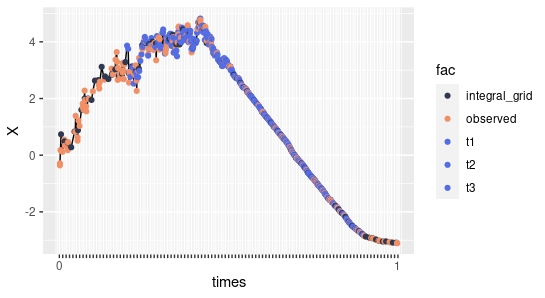
\includegraphics[width=0.48\textwidth]{Images/simul/all.jpeg}
	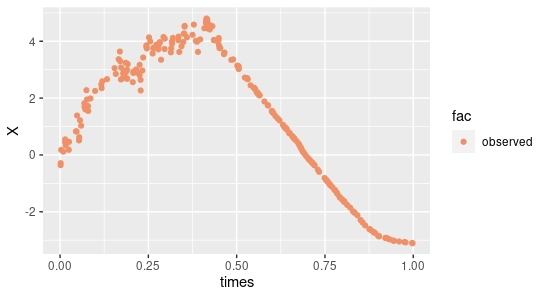
\includegraphics[width=0.48\textwidth]{Images/simul/observed.jpeg}

	\textbf{Lissage des données}

	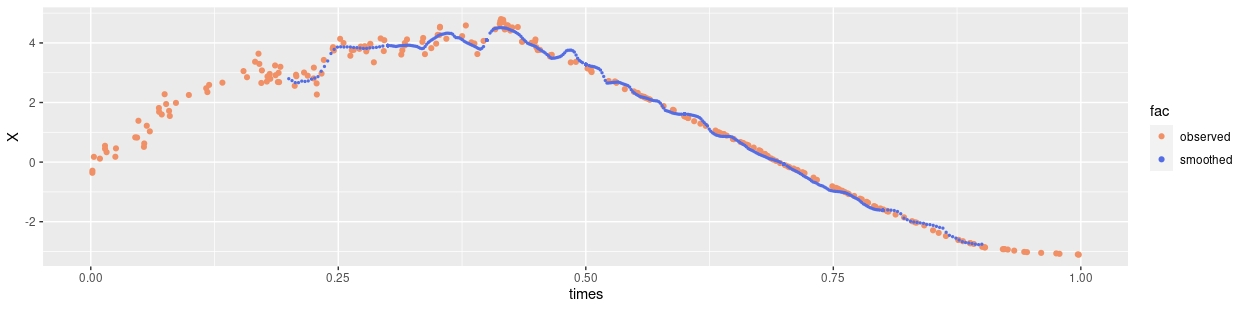
\includegraphics[width=0.96\textwidth]{Images/simul/smoothed.jpeg}
	\caption{Visualisation des données générées : $\lambda = 255, N = 200,$ 30 valeurs de $\Delta$}
\end{figure}


\subsection{Pré-Lissage}

Le pré-lissage des courbes a été fait en utilisant un lissge non paramétrique à noyaux\footnote{ainsi qu'un lissage utilisant des splines pénalisées, et des ondelettes mais on ne se concentrera sur les autres lissages qu'en Annexe \ref{annexe:prelissage_impact}}. Comme mentionné dans la section \ref{eq:h_cross_noyau_pre}, chaque courbe est lissée en utilisant une fenêtre par validation croisée avec la grille $\mathcal H= \{ 0.01 \dots 0.2 \}_{50}$ avec pour métrique une estimation du risque quadratique $\esperance{|\widehat Y_{(-i)} - Y|^2}$. On ne regarde pas de fenêtre au delà de $\Delta = 0.2$ car il serait difficile de justifier pour l'estimation de la régularité que l'on lisse en regardant plus de $20$\% du support alors que la régularité évolue sur l'ensemble de l'intervalle.

L'obtention de la fenêtre de lissage a été réalisée en réalisant une validation croisée sur une grille de fenêtre étalées sur une échelle de puissance entre $h_{min} = 2 / \widehat \lambda$ et $h_{max} = 1 / \widehat \lambda^{1/3}$.

\begin{align*}
	                                                 & \mathcal H = \bigl\{ h_k, \, k \in \llbracket 1, K \rrbracket \bigr\}
	\\
	\forall k \in \llbracket 1, K \rrbracket, \qquad & h_k = h_{min} e^{ - a \cdot k }
	\\
	\text{avec } \qquad                              & a = \frac{\log \left( h_{max} \right) - \log(h_{min})}{K}
	\\
	\textsf{de valeur max} \qquad                    & h_K = h_{max} = h_{min} e^{ - a \cdot K }
	\\
	\text{et } \qquad                                & K = 30
\end{align*}

Cela est dû au fait que $h^*_{\mathcal R_{\textsf{quadr}}} = \grandop{ \lambda^{- \frac 1 {1 + 2H_t}} }$ avec $0<H_t<1$, comme vu dans la section \ref{sec:regloc-prelissage}. De plus, on souhaite que dans notre fenêtre de lissage, en moyenne, se trouvent 2 points au minimum. 




% \section{Qualité de l'estimation des incréments quadratiques moyens}
% 
\newcommand{\thetaA}{\Theta_{1 \rightarrow \overset{3}{\underset {2}{}}}}
\newcommand{\cindexA}{_{1 \rightarrow \overset{3}{\underset {2}{}}}}
\newcommand{\thetaB}{\Theta_{\overset 1{\underset{2}{ }} \rightarrow3}}
\newcommand{\cindexB}{_{\overset 1{\underset{2}{ }} \rightarrow3}}
\newcommand{\thetaC}{\Theta_{1 \rightarrow 2 \rightarrow 3}}
\newcommand{\cindexC}{_{1 \rightarrow 2 \rightarrow 3}}
\newcommand{\notequiv}{\overset {\textsf{\faTimes}} \iff}
\newcommand{\yesequiv}{\overset {\textsf{\faCheck}} \iff}

Il y a différentes manières de définir les paramètres de régularité $\hat H_t$ et $\hat L_t$. En effet il est possible de définir $\hat H_t$ en utilisant $\hat \theta (t_1, t_2)$ mais aussi en utilisant $\hat \theta (t_2, t_3)$ ($\theta(t_1, t_3)$ est forcément utilisé\footnote{$\hat H_t$ ne serait même pas bien défini pour le couple $\theta(t_1, t_2)$, $\theta(t_2, t_3)$}). De même pour $\hat L_t$. On peut donc se demander quels sont les meilleurs $\theta(u,v)$ avec $u,v \in \{t_1, t_2, t_3\}$ à utiliser pour obtenir la meilleure estimation de $H_t$ et $L_t$ ainsi que leur $\Delta$ optimal associé pour l'estimation de ces paramètres.

\bigskip

Le problème est que le proxy $\theta$ est défini comme une espérance, et donc n'est pas observable. On ne peut donc pas directement comparer $\hat \theta(u,v) = \sum_i|\widehat X_i(u) - \widehat X_i(v)|^2$ et $\theta(u,v) = \esperanceloi X { |X(u) - X(v)|^2 }$, à moins d'avoir fait le calcul de l'expression explicite en connaissant la loi du processus initial.

\bigskip

On peut cependant comparer $\hat \theta(u,v)$ et $\widetilde \theta(u,v) = \frac 1 N \sum_i |X_i(u) - X_i(v)|^2$ qui est un estimateur de $\theta(u,v)$, et que l'on obtient aisément avec la simulation. On peut ainsi déterminer pour quelle valeur de $\Delta$ et quel couple $(u,v)$ on dispose de la meilleur estimation du $\tilde \theta$, qui est entre-autre le meilleur estimateur que l'on pourrait espérer de $\theta$. Le meilleur couple (au sens donné dans cette section) est pris comme étant les deux $\hat \theta(u,v)$ réalisant les risques minimaux par rapport au $\tilde \theta$ sur les 3 couples $(u,v)$ possibles.

\begin{table}[H]
	\centering
	\begin{tabular}{l|ll|}
		\cline{2-3}
		                                     & $\lambda < 120$                                                                                            & $\lambda \geq 120$                                                                 \\ \hline
		\multicolumn{1}{|l|}{$H_t < 0.6$}    & \multicolumn{1}{l|}{\begin{tabular}[c]{@{}l@{}}$\thetaC$\\ \\ \\ $\Delta^- \rightarrow 0.01$\end{tabular}} & \begin{tabular}[c]{@{}l@{}}$\thetaA$\\ \\ $\Delta^+ \rightarrow 0.2$\end{tabular}  \\ \cline{2-3}
		\multicolumn{1}{|l|}{$H_t \geq 0.6$} & \multicolumn{1}{l|}{\begin{tabular}[c]{@{}l@{}}$\thetaA$\\ \\ $\Delta^- \rightarrow 0.2$\end{tabular}}     & \begin{tabular}[c]{@{}l@{}}$\thetaC$\\ \\ $\Delta^+ \rightarrow 0.01$\end{tabular} \\ \hline
	\end{tabular}
	\caption{Tableau récapitulatif des $\Theta$ optimaux : Risque individuel sur $\tilde \theta(u,v)$}
	\label{tab:recap_theta_single}
\end{table}

% 
% \section{Qualité de l'estimation de la régularité locale}
% 
Les simulations de Monte Carlo permettent d'avoir accès directement à la véritable régularité de la courbe en chaque point. Nous allons dans l'étude du comportement du $\Delta$ essayer de tirer profit de cet avantage que ne possède pas le praticien qui utilise des données réelles.


\begin{table}[H]
    \centering
    \begin{tabular}{l|ll|}
        \cline{2-3}
                                              & $\lambda < 120$                                                                                                                                                                                                    & $\lambda \geq 120$                                                                                                                                        \\ \hline
        \multicolumn{1}{|l|}{$H_t \leq 0.65$} & \multicolumn{1}{l|}{\begin{tabular}[c]{@{}l@{}}$\yesequiv \mathcal R$\\ $\yesequiv \Delta^*$\\ $\Delta^- \downarrow 0.01$\end{tabular}}                                                                            & \begin{tabular}[c]{@{}l@{}}$\simeq \yesequiv \mathcal R$\\ $\notequiv \Delta^*$\\ $\Delta^+ \rightarrow [\leq 0.6] 0.1/0.2 [\geq 0.6]$\end{tabular}        \\ \cline{2-3}
        \multicolumn{1}{|l|}{$H_t > 0.65$}    & \multicolumn{1}{l|}{\begin{tabular}[c]{@{}l@{}}$\yesequiv \mathcal R$\\ $\notequiv \Delta^*$\\ \faExclamationTriangle $H=0.7 : \Delta^- = 0.02$\\ \faExclamationTriangle $H = 0.73 : \Delta^- = 0.2$\end{tabular}} & \begin{tabular}[c]{@{}l@{}}$\thetaA$\\ \faExclamationTriangle $H=0.7 : \Delta^+ = 0.02$\\ \faExclamationTriangle $H = 0.73 : \Delta^+ = 0.2$\end{tabular} \\ \hline
    \end{tabular}
    \caption{Tableau récapitulatif des $\Delta$ optimaux : Risque sur $H_t$}
    \label{tab:recap_delta_H}
\end{table}

\section{Détermination du $\Delta$ optimal à choisir pour l'estimation de la régularité}

\noindent L'étude des courbes de risques obtenues :

\begin{equation*}
\widehat{\mathcal R} \bigl( \, \Theta \, , \, \Delta \, \bigr) 
= 
\frac 1 {mc} \sum\limits_{p=1}^{mc} \frac{{\distnorme 2 {\widehat \Theta\bigl[\, p \,\bigr]} {\widetilde \Theta \bigl[ \,p \,\bigr]}}^2}{{\norme 2 {\widetilde \Theta \bigl[ \,p \,\bigr]}}^2}
\end{equation*}

indiquent la sélection du $\Delta$ par la procédure suivante\footnote{Des détails sur la détermination de la procédure de sélection du $\Delta$ en annexe \ref{annexe:choix_risque_couple}} :

\begin{itemize}
	\item \textbf{Détermination de la fenêtre de pré-lissage :}
	\begin{itemize}

		\item Il est important de prendre en compte les \og trous \fg lors du lissage à noyau des courbes. Il convient donc de ne pas sélectionner les fenêtres de lissage où le lissage à noyau a échoué sur une partie du support. On pourra se référer à l'annexe \ref{annexe:lissage_fail} pour plus de détails.

		\item Pour les données \textbf{sparses} en nombre moyen d'observations par courbe ($\widehat \lambda \leq  100-150$) : Bien lisser les courbes individuellement en déterminant la fenêtre de lissage par validation croisée.
	\end{itemize}


	\bigskip

	\item \textbf{Choix du couple :}

	\begin{itemize}
		\item \textbf{on dispose d'une information a priori sur une idée des zones plus ou moins régulières de données :} Il est conseillé d'estimer le couple dont la deuxième composante (c'est à dire soit $\theta_{12}$ soit $\theta_{23}$) est celle qui pointe vers l'information la plus régulière. Même si les risques entre les couples $\thetaA$ et $\thetaB$ étaient proches, celui qui utilisait $\theta_{23}$ était souvent meilleur. Et-ce, que ce soit pour le risque relatif ou le risque absolu d'ailleurs. Dans le cadre de notre simulation $\theta_{23}$ correspondait à l'information plus régulière (car $t \mapsto H_t$ était croissante).
		\item \textbf{On ne dispose d'aucune information à priori sur la régularité :} Les deux couples ne disposent pas d'un risque qui diffère grandement ($cf$ graphiques \ref{fig:sparse_osef_rel})
	\end{itemize}

\bigskip

\item \textbf{Choix du $\Delta$ : } En se référant aux graphiques en annexe \ref{fig:sparse_osef_rel}, on recommande l'utilisation d'un $\Delta$ relativement grand vis-à-vis du support. Les graphes des risques indiquent que les $\Delta$ de la taille de 10 à 20\% du support étaient à risques relatifs équivalents, et ce pour les différents niveaux de régularité (0.5 à 0.7). C'est pourquoi dans l'optique d'une estimation de la régularité \og locale \fg on recommande plutôt de se situer aux environs de 15-20\% du support pour bénéficier du plateau autour, tout en restant local, étant donnée que les données simulées avaient une régularité qui ne variait pas brusquement sur le support.

\bigskip

\item \textbf{Si l'on tient au risque euclidien (non relatif) : } Il est recommandé pour le risque euclidien non relatif après avoir analysé les graphes \ref{fig:compare_xtrm_2} en ayant retiré les points extrêmes, de prendre un $\Delta$ proche de $0.01$ pour les zones moins régulières ($H_t < 0.6$) et $\Delta$ proche de $0.2$ pour les zones plus régulières ($H_t \geq 0.6$). Si l'on ne possède aucune information, il est possible d'effectuer un premier lissage qui estime la régularité avec $\Delta = 0.01$\footnote{Lorsque $\Delta = 0.2$ est optimal, pour le risque euclidien non relatif à la norme de la cible, $\Delta = 0.01$ n'engendre pas —dans le cadre de la simulation— la pire valeur de risque possible, là où 0.2 donne le pire risque lorsque $0.01$ est optimal. Il est donc plus prudent d'effectuer une première estimation avec $\Delta = 0.01$.}, puis avec cette estimation ré-effectuer un lissage en évaluant cette fois la régularité avec le $\Delta$ qui aura été recommandé dans cette section pour le risque euclidien (non relatif).
\end{itemize}

\section{Discussion}

Il est à noter que le choix du risque apportait une conclusion différente sur la détermination de $\Delta$ à choisir en pratique. Le choix du risque euclidien relatif à la norme de la cible semblait être un choix qui fait plus sens à la fois d'un point de vue méthodologique, mais aussi par chance, un choix qui mène à une règle de détermination assez simple du $\Delta$ avec une courbe de risque qui semble mieux se comporter. 

\bigskip

On pourra noter aussi les différents pics présents à certaines valeurs de $\Delta$ dans les graphes de risque. Après investigation des courbes des réplications de monte-carlo présentant des cas extrêmes ( comme par exemple un risque euclidien non relatif s'élevant jusqu'à 80 — comme sur la figure \ref{fig:dist_R_eucl_curves} ), Il semblerait que cela soit dû à l'estimation de $X(t_1), X(t_3)$ non loin, ou bien même dans un \og trou d'observation \fg. Le praticien doit donc faire attention lors de l'estimation de la régularité si il obtient des résultats peu concluants, si les courbes initiales possèdent peu de points (ou pas de points) proches des temps $t_1(\Delta), t_2(\Delta)$ ou $t_3(\Delta)$. Auquel cas, pour estimer la régularité deux pistes se présentent :

\begin{itemize}
\item estimer la régularité par les statistiques d'ordre, pour le voisinage des points problématiques via la méthode de Golovkine et al.

\bigskip

\item Investiguer sur le potentiel de lisser via une base de fonction, qui ne détruit pas trop les informations de régularité, comme la base d'ondelettes. Ce qui rend la base d'ondelettes particulièrement intéressante est explicité en annexe \ref{annexe:wavelet}.
\end{itemize}
